\chapter{Idee ontwikkeling}
\label{cha:ideeOntwikkeling}
\textit{In dit hoofdstuk is de opzet gemaakt voor het maken van het meubel hondje. Hier zijn verschillende ontwerp methodes toegepast (\cref{se:creatief_proces}), deel concepten (\cref{se:Deelontwerpen}), spuug modellen (\cref{se:Spuugmodellen}) en ook drie kansrijke totaalconcepten (\cref{se:totaalconcepten}).}


\section{Creatief proces}
\label{se:creatief_proces}
{\bf In de eerste weken zijn er brainstormsessies gehouden om oplossingen te vinden op de deelfuncties.}
\subsection{ACCREx}
Tijdens het ontwerpproces is er gebruik gemaakt van diverse methodes voor het bedenken van ideeën. Ook is er gebruik gemaakt van ACCREx, (\cite{coelho_2011}), hier is voor gekozen omdat hier een aantal interessante mogelijkheden lagen voor het toepassen van ACCREx.\\
Bij deze ontwerpopdracht was het van belang om een oplossing te bedenken om over het talud te komen. Daarom is er voor gekozen om bij dit ontwerp probleem ACCREx toe te passen. ACCREx is toegepast door 2 manieren van voortbewegen tegen elkaar uit te zetten en te kijken of er daar ideeën uit kunnen worden gehaald. Er is gekozen om horizontale verplaatsing tegen verticale verplaatsing uit te zetten. Deze combinatie van manieren gaf een frame waarin ideeën konden worden bedacht. \\

\subsection{Bio inspired design}
Tijdens het ontwerp proces is er ook gekeken naar alternatieve vormen van ideeën en oplossingen generen, zoals bio-inspired design. De opgave was een paar voorbeelden van de natuur te bedenken die het zelfde probleem heeft moeten over overwinnen.
\vspace{\baselineskip}

\textbf{Duizendpoot.} Na onderzoek kwam al snel een duizendpoot naar voren. Het interessante van een duizend poot verraad de naam al, de hoeveelheid pootjes. Wanneer er een groot aantal pootjes wordt toevoegt in een mechanisme is het in staat om voort te bewegen op een manier waarbij het lijkt alsof het rolt. Het probleem van een lopend mechanisme is dat het moeilijk is om het pakketje recht te houden. Dit wordt opgelost door middel van veel pootjes, daarom is de duizendpoot interessant in dit onderzoek. Ook blijft de duizendpoot overeind als niet alle poten zich op de grond bevinden. Dit principe kunnen we goed gebruiken voor ons concept.\\

\vspace{\baselineskip}
{\bf Kruiper.} De rups was een voorbeeld dat al snel naar boven kwam. De rups maakt gebruik van het feit dat hij zijn lichaam kan intrekken en kan uitrekken. Door zich vast te klemmen met het voorste gedeelte van zijn lichaam kan hij het achterste deel naar zich toe trekken als het ware. Om zich dan voort te bewegen zet hij zijn achterkant vast en drukt als het ware zijn lichaam naar voren, hij rekt zich dan uit.
\vspace{\baselineskip}
\\
{\bf Hopper.} Ook de sprinkhaan en de haas kwamen na verder onderzoek naar voren. Deze twee organismes maken gebruik van hun krachtige achterpoten om niet te lopen maar te springen als het ware. Relatief kleine obstakels zijn voor deze wezens geen probleem omdat zij er gewoon over heen springen. Dit zou wellicht kunnen toe worden gepast in het ontwerp project.
\vspace{\baselineskip}
\\
{\bf Mantis car.} Het laatste idee wat werd gegenereerd door de groep was een 'mantis-car'. Dit concept is gebaseerd op hoe een sprinkhaan zijn poten gebruikt om zijn prooi vast te grijpen. Ook is de vorm van de poten cruciaal geweest voor het concept. Het principe 'mantis-car' is eigenlijk het vastklemmen met mechanische poten op het obstakel en de rest van het voertuig zich hierdoor omhoog te hijsen.\\
\vspace{\baselineskip}

\subsection{Morfologische kaart}
Door op verschillende manieren te brainstormen zijn er diverse oplossingen voor elke deel functie gevonden. Deze zijn samengebracht in een morfologische kaart (\cite{toolbox_voor_ontwerpers_ipo_windesheim}). Deze kan worden gevonden in \cref{ap:bijlage_A}. \\


\section{Deel ontwerpen}
\label{se:Deelontwerpen}
Om tot kansrijke concepten te komen, heeft elk groepslid een combinatie van oplossingen uit de morfologische kaart (zie \cref{ap:bijlage_A}) uitgewerkt tot een totaaloplossing. Het doel hier van is om concreter na te denken over hoe deeloplossingen samen kunnen werken. Zo kunnen zwakke plekken in elk ontwerp later als spuugmodel uitgewerkt worden en in het uiteindelijke ontwerp geïntegreerd worden.\\
\vspace{\baselineskip}

{\bf Schuiver.}
De schuiver maakt gebruikt van twee schaarliften en een uitschuif systeem. Aan de twee schaarliften zijn wielen verbonden die worden aangedreven, hiermee kan het systeem zichzelf voortbewegen. De schaarliften hebben twee functies, ten eerste zorgen ze ervoor dat het hoogteverschil van het pakketje kan worden bereikt. De tweede functie van de schaarliften is het overbruggen van de obstakel. Als één schaarlift opklapt terwijl de ander open blijft, kan de wagen met een stappende beweging over het obstakel heen 'lopen'. \\

\vspace{\baselineskip}
{\bf Inklapper.}
De inklapper is gebaseerd op het principe van inklapbare pootjes. Het ontwerp heeft 4 paar pootjes die allemaal in het verlengde van zichzelf kunnen inklappen. De inklapper is aangedreven door een verbrandingsmotor. De vier wielen aan de linkerkant zijn onafhankelijk van de vier wielen aan de rechter kant aangedreven. Dit zorgt ervoor dat hij zichzelf kan sturen door een kant van de wielen te laten rijden en de andere kant te laten remmen. De inklapper neemt het talud door zijn pootjes erop te laten botsen en dat ze dan inklappen. als de pootjes er weer over zijn klappen ze weer uit. Dit gebeurt met alle vier de paren zodat het mechanisme erover heen kan komen zonder het pakket te laten kantelen. Zie voor meer informatie \cref{fig:inklapper_tekening}. \\

\begin{figure}[H]
    \centering
    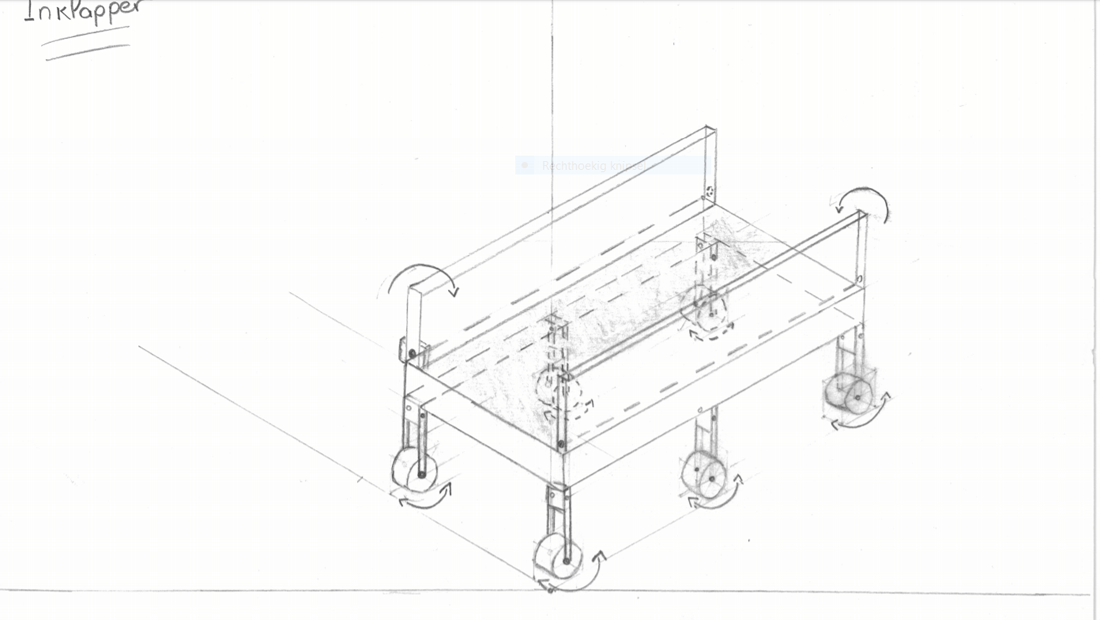
\includegraphics[width = 100mm]{04_idee_ontwikkeling/Inklapper,_deelontwerp_Beer.PNG}
    \caption{Tekening van het deelconcept inklapper.}
    \label{fig:inklapper_tekening}
\end{figure}

\vspace{\baselineskip}
{\bf Fietskar}. Dit concept maakt gebruik van een schaarlift dat het systeem omhoog brengt. Hierdoor hebben de voorste en achterste wielen geen contact meer met de grond. Vervolgens rijdt het karretje zijn voorste wiel over het talud. Eenmaal met zijn voorste wiel over het talud trekt hij zijn schaarlift in rijdt hij zijn schaarlift er overheen. Deze beweging wordt herhaald om de achterste wielen over het talud te krijgen. Het sturen doet hij met een fietswiel mechanisme wat aangedreven wordt door een fietsstuur. De fietsstuur wordt aangedreven met een servomotor die op afstand kan worden bestuurd Voor meer informatie zie \cref{fig: fietscar}.

\begin{figure}[H]
    \centering
    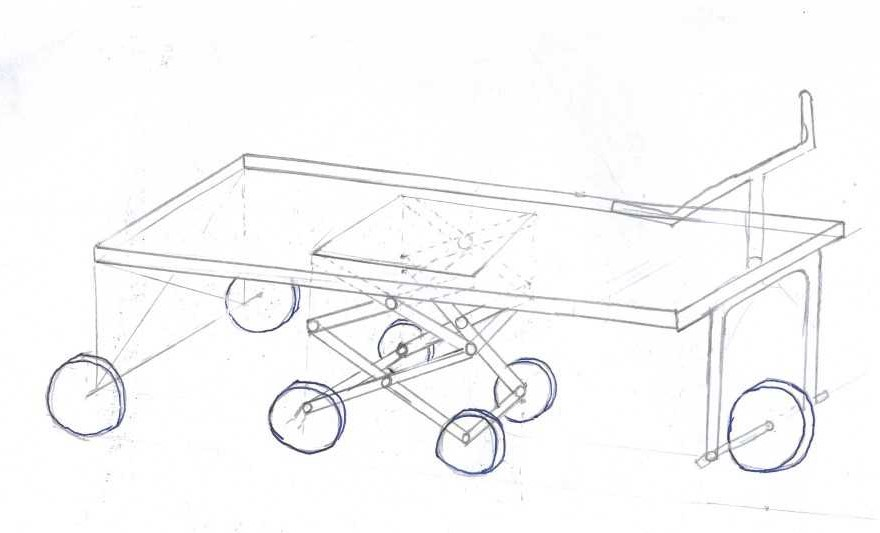
\includegraphics[width = 80mm]{04_idee_ontwikkeling/Deelontwerp-Kevin.jpeg}
    \caption{Tekening van deelconcept fietscar}
    \label{fig: fietscar}
\end{figure}

\vspace{\baselineskip}
{\bf Haaktank} De haaktank maakt gebruik van grote rupsbanden om over het talud heen te komen een een grijphaak om grotere obstakels te overwinnen. Het wordt aangedreven door elektromotoren en wordt radiografisch bestuurd. Het pakket wordt met spanbanden bevestigd zodat het stabiel blijft tijdens transport. Voor een isometrische tekening zie \cref{fig:Haaktank}.


\begin{figure}[H]
    \centering
    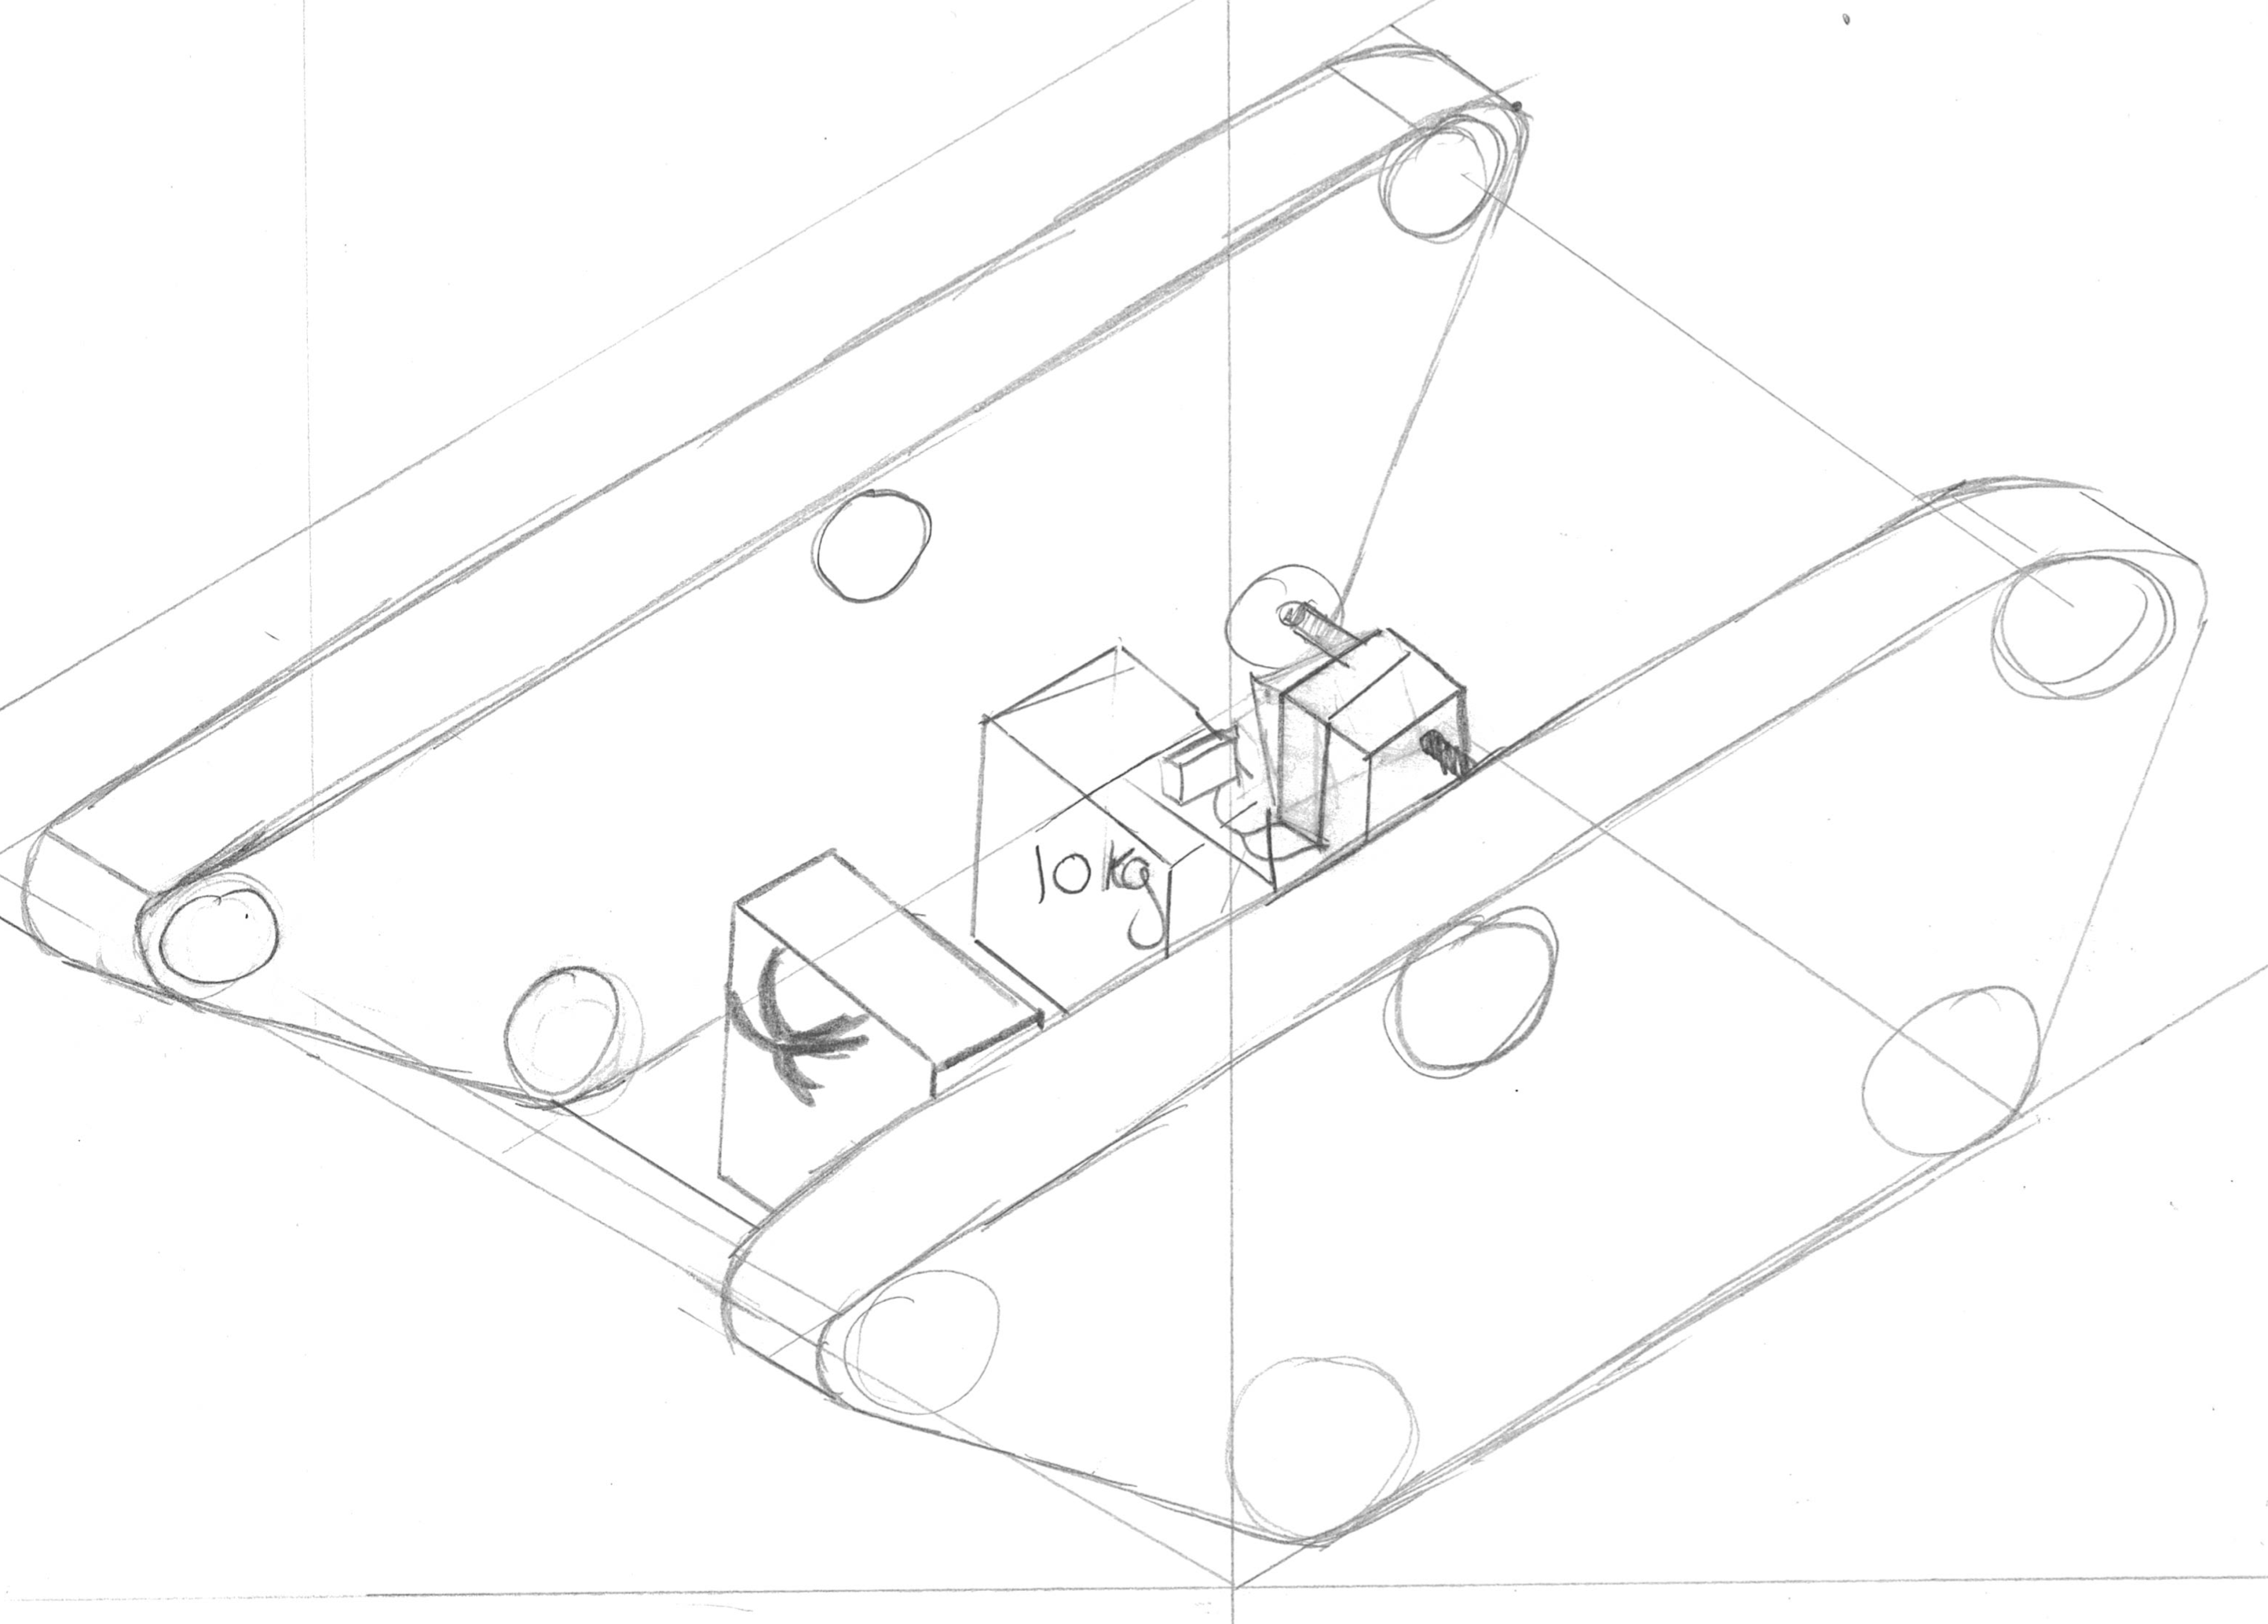
\includegraphics[width = 60mm]{04_idee_ontwikkeling/Deel_ontwerp_robin.png}
    \caption{Isometrische tekening van de Haaktank}
    \label{fig:Haaktank}
\end{figure}


    
\vspace{\baselineskip}
{\bf Strand beest.} 
Het strand beest maakt gebruik van een 4-stangen mechanisme om te lopen, hierdoor is hij in staat om over de hindernissen te stappen. Hij kan op gelijke hoogte komen met het pakketje door middel van een schaarlift. door de omsluitende wanden kan het pakketje niet vallen. Om het pakketje af te geven heeft het een klepje die open kan aan de voorkant om het pakketje er weer uit te schuiven. Hij stuurt door onafhankelijke aandrijving. De 4 stangen worden aangedreven door een elektromotor. Voor een beter beeld zie \cref{schaarlift_hilbert}.

\begin{figure}[t]
    \centering
    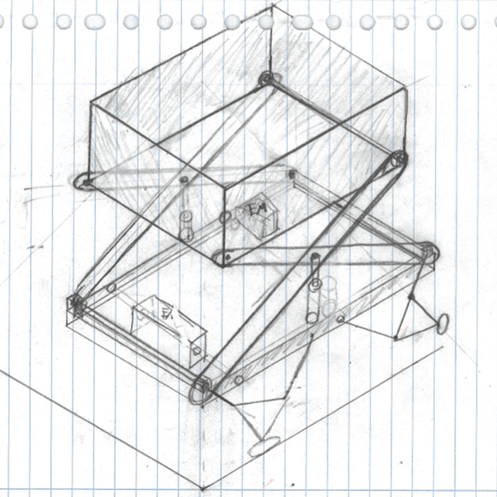
\includegraphics[width = 100mm]{04_idee_ontwikkeling/Deeloplossing_schaarlift,_Hilbert_(1).PNG}
    \caption{Tekening van deelconcept strandbeest}
    \label{schaarlift_hilbert}
\end{figure}

{\bf Mantistank}. 
De mantistank is gebaseerd op onafhankelijke aandrijving en overkomt de taluds d.m.v. de grijphaken, zie \cref{mantistank_max} Er is onafhankelijke aandrijving gerealisserd door stepper motoren. De 2 rupsbanden hebben allebei een eigen as zodat er geen differentiaal is en de onafhankelijke aandrijving gebruikt kan worden om te sturen. Het concept kan obstakels overkomen door middel van een soort grijp systeem, waarom dit concept ook wel de ‘mantis-car’ wordt genoemd, alias de mantis in de natuur. Het pakketje wordt opgevangen en ingesloten door middel van het pakket op het wagentje te schuiven, waarna er een drukplaat naar beneden wordt gedrukt waardoor de wanden insluiten door middel van trekveren. Dit laatste is alleen niet aangegeven op de tekening. \\
\vspace{\baselineskip}

\begin{figure}[H]
    \centering
    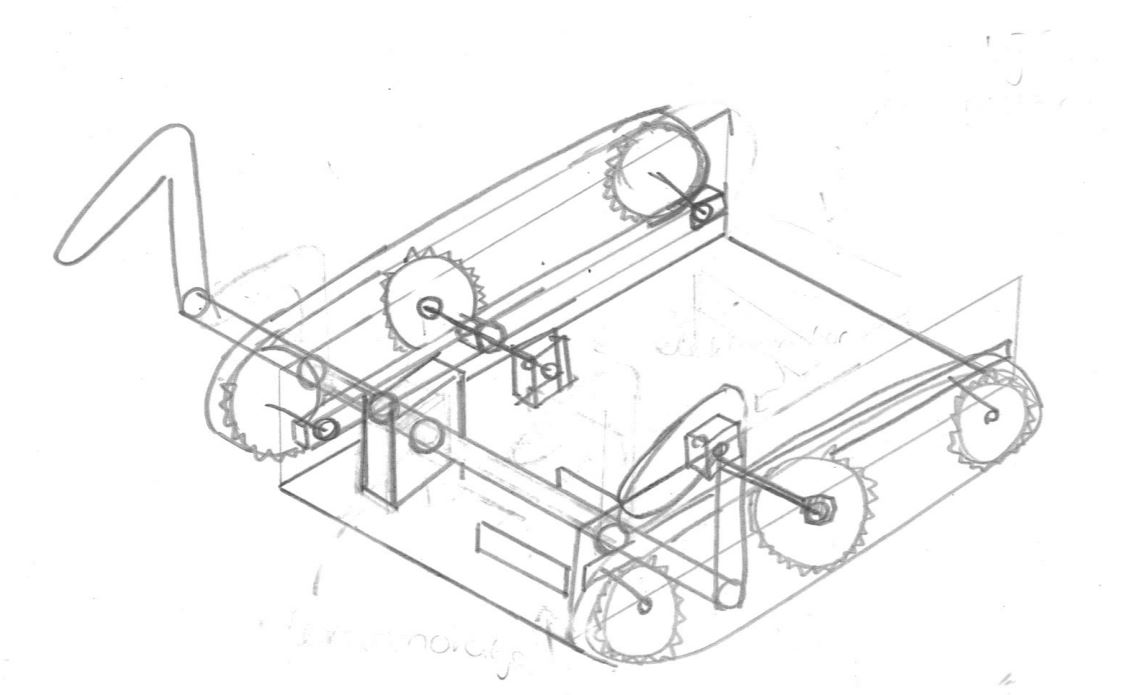
\includegraphics[width = 100mm]{04_idee_ontwikkeling/deelconcept_mantistank.JPG}
    \caption{Tekening deeloplossing mantistank}
    \label{mantistank_max}
\end{figure}

\section{Spuugmodellen}
\label{se:Spuugmodellen}
\vspace{\baselineskip}
Tijdens het ontwerpfase is het van groot belang dat er spuugmodellen worden gemaakt om beter inzicht te krijgen op de werking van de mechanismen. Vanuit de morfologische kaart zijn er een aantal spuugmodellen, waarvan de meest kansrijke vervolgens zijn uitgewerkt tot een werkelijk deeloplossing. 
\subsection{gekozen spuug modellen}
\vspace{\baselineskip}

{Om zo veel mogelijk inzicht te krijgen in de mogelijkheden om verschillende ontwerpproblemen aan te pakken is ervoor gekozen om een aantal spuugmodellen te maken.} \\

\begin{description}
\item[A.] {\bf Schaarlift.}\\ 
Het eerste gekozen spuugmodel is een model van een schaarlift. Het doel van het maken van een schaarlift was om te kijken waar eventuele veren moesten worden geplaatst en hoe de schaarlift optimaal zou werken.  Voor meer informatie zie \cref{fig:plaatje_schaarlift}.

\begin{figure}[H]
\centering

    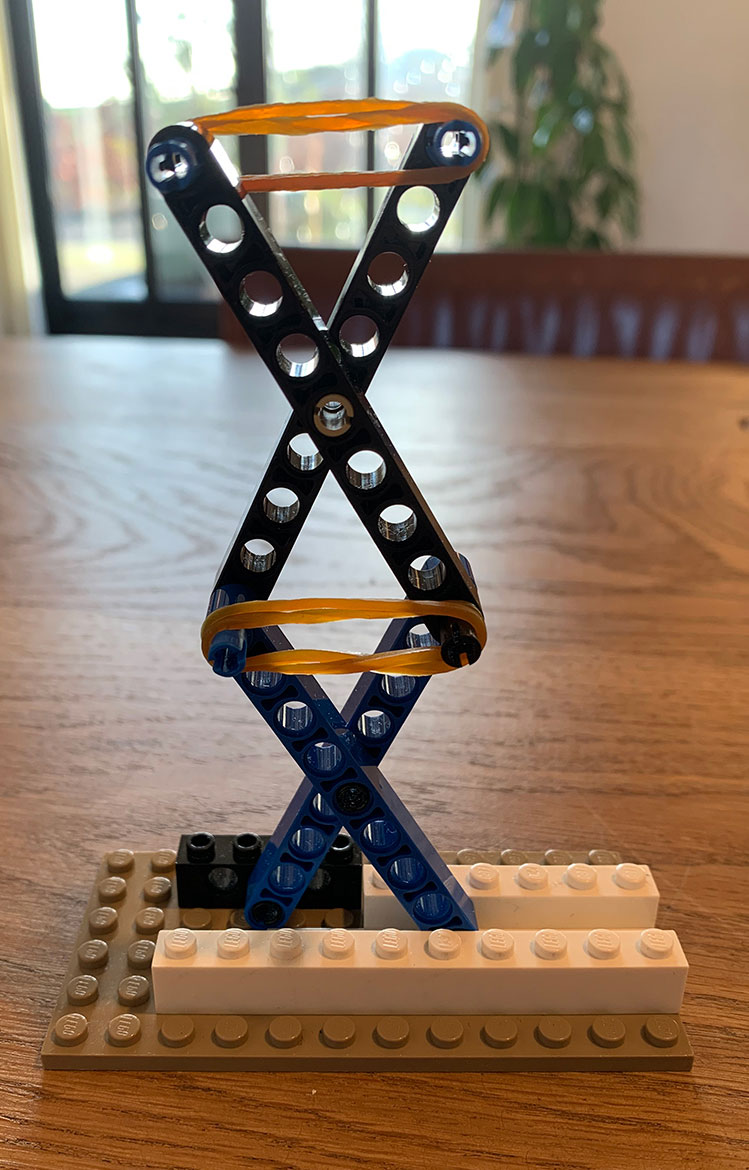
\includegraphics[width = 50mm, angle =270 ]{04_idee_ontwikkeling/IMG_0892.jpg}
    \caption{Spuug model schaarlift}
    \label{fig:plaatje_schaarlift}
\end{figure}

\vspace{\baselineskip}

\item[B.] {\bf Inklap wielen.}\\
Het is een interessant spuugmodel omdat het gebruik van inklapwielen een kansrijke deeloplossing is en het essentieel is om dan vroeg achter de ontwerp uitdagingen van zo 'n inklap wiel te komen. Het spuugmodel is uit lego gemaakt omdat dit makkelijk te assembleren was en er veel verschillende manieren zijn om het te maken zodat er ook kon worden gekeken naar hoe het optimaal kon worden gedaan. Voor meer informatie zie \cref{fig:inklapwielen}. \\

\begin{figure}[H]
\centering

    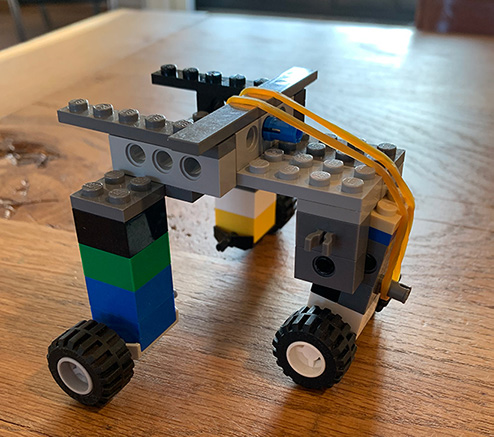
\includegraphics[width = 50mm, angle = 270]{04_idee_ontwikkeling/Inklapwielen.jpg}
    \caption{Spuug model inklapwielen}
    \label{fig:inklapwielen}
\end{figure}

\item[C.] {\bf Mantis klauwen.}\\
De mantis klauwen zijn relatief makkelijk te construeren en te assembleren op een frame. Hierdoor is het een interessant spuugmodel omdat het wellicht makkelijk is om dit spuugmodel te perfectioneren. Het leek de groep ook essentieel om te onderzoeken hoe lang de klauwen van zo'n mantis systeem moesten zijn voordat het werkte. In \cref{fig:Mantis_spuug} is een spuugmodel van de Mantis Car afgebeeld. \\

\begin{figure}[H]
\centering
    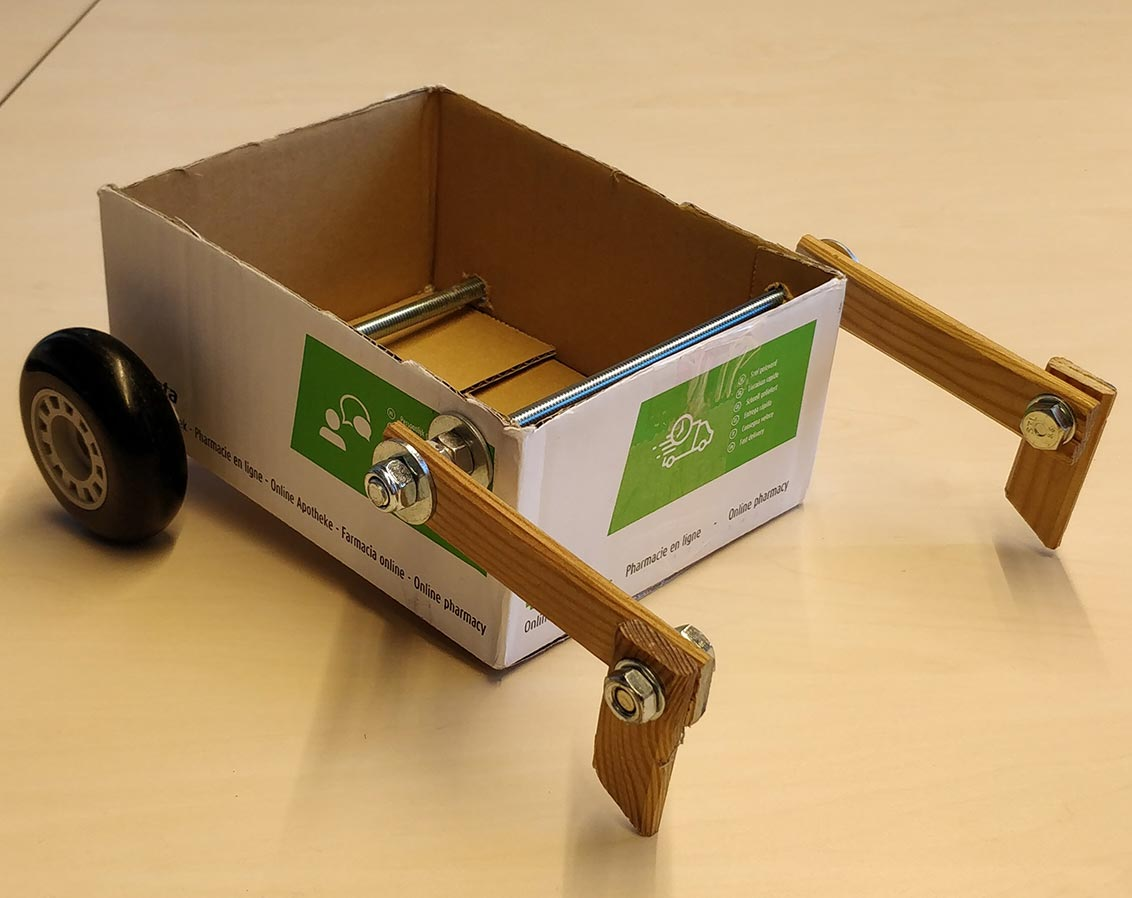
\includegraphics[width = 50mm]{04_idee_ontwikkeling/Mantis_spuugmodel.jpg}
    \caption{Spuugmodel Mantis Car}
    \label{fig:Mantis_spuug}
\end{figure} 

\item[D.] {\bf Stuursysteem.}\\
Er werd ook gekeken naar verschillende stuursystemen, wat werkt en wat niet werkt. Daarom is er gekozen voor het maken van een stuursysteem dat lijkt op het sturen van een fietswiel. Dit sturen wordt gerealiseerd door middel van een servo. (zie \cref{fig:Fietsstuur}). \\

\begin{figure}[H]
    \centering
    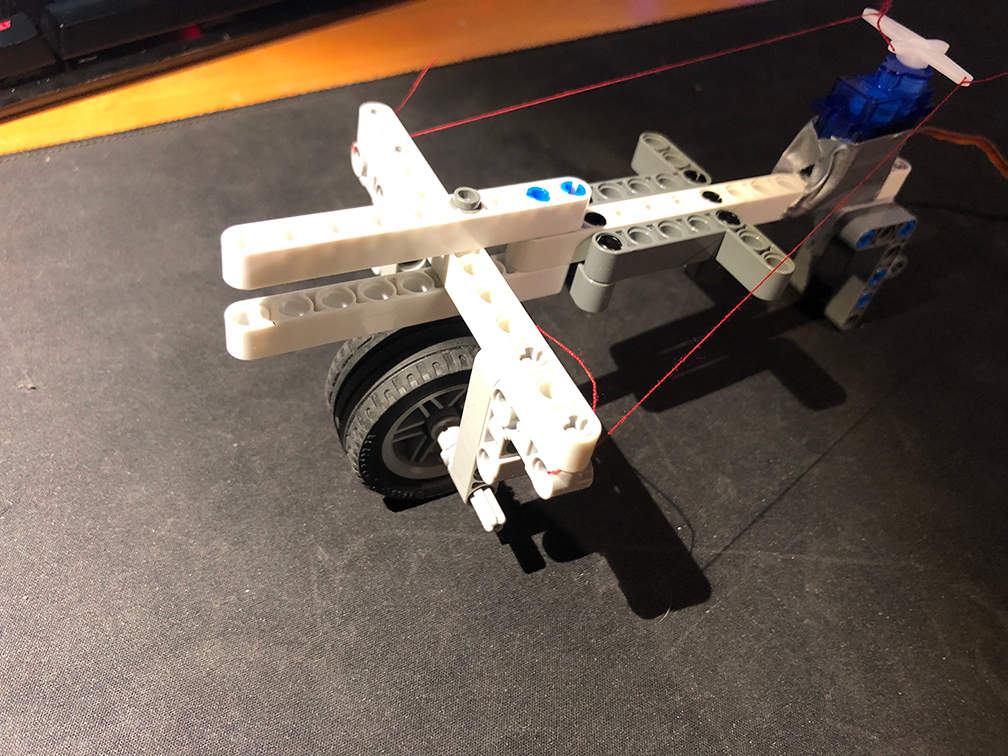
\includegraphics[width = 50mm]{04_idee_ontwikkeling/fietsstuur.jpg}
    \caption{Spuugmodel Stuurssysteem}
    \label{fig:Fietsstuur}
\end{figure} 



\item[E.] {\bf Radiografische besturing.}\\
In verschillende deel ontwerpen wordt er gebruik gemaakt van radiografische besturing. Het is belangrijk om te weten hoe deze radiografische besturing gerealiseerd kan worden voordat het toegepast wordt in een ontwerp. Radiografische besturing bleek niet moeilijk te realiseren te zijn. Zie \cref{fig:arduino}.


\begin{figure}[H]
    \centering
    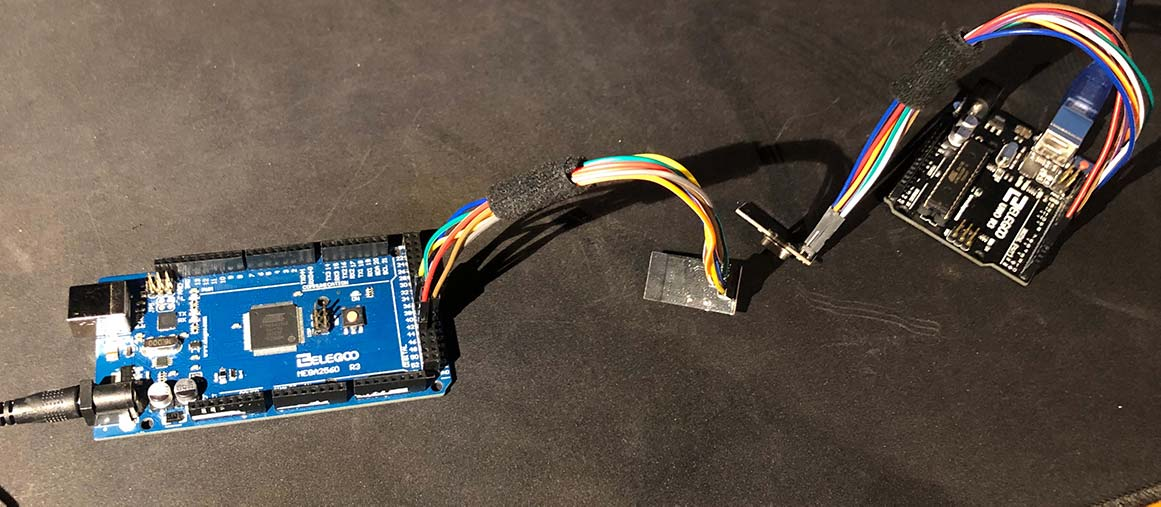
\includegraphics[width = 80mm]{04_idee_ontwikkeling/RC_arduinos.jpg}
    \caption{Arduino's communicerend over radiosignalen.}
    \label{fig:arduino}
\end{figure} 


\end{description}

%%veel plaatjes, met onderschrift dat past bij verwijzing naar foto's, (zie tekst)

\subsection{Evaluatie spuug modellen}
\vspace{\baselineskip}

\begin{description}

\item[A.] {\bf Schaarlift.}\\
De schaarlift is een relatief makkelijk principe als het gaat om fabricage en werking. Toch zijn er een aantal complicaties gevonden waar nog oplossingen voor moesten worden gevonden. \\
Een probleem van de schaarlift is de aandrijving ervan. Om de schaarlift te laten in klappen moeten de twee uiteinden van de schaarlift zich van elkaar af bewegen. Dit kan worden gerealiseerd worden door middel van een roterende as met een touwtje die zich opwindt en zo een van de uiteinden weg trekt. Dit kan ook worden opgelost door een tandheugel. Het probleem hiervan is dat ervoor gezorgd moet worden dat het tandwiel op de tandheugel moet blijven. \\
Nog een probleem van een schaarlift is de verplaatsing van de uiteinden. Doordat de uiteindes zich van elkaar af bewegen kunnen ze niet worden vastgeklemd. De uiteindes mogen een graad van vrijheid hebben, zodat ze wel horizontaal van elkaar af kunnen bewegen. \\ 

\item[B.] {\bf Inklap wielen.}\\
De inklapbare wielen was een makkelijk te maken spuug model, maar het gaf veel inzicht. \\ 
Een van de voordelen van inklapbare wielen is dat  het op veel verschillende manieren kan worden toegepast. Het is namelijk mogelijk om de wieltjes via een mechanische aandrijving in te laten klappen en uit te laten klappen. Dit zorgt ervoor dat het pakket hondje in principe het talud niet aan hoeft te raken. Het voordeel hiervan is dat het pakket hondje allerlei soorten obstakels kan nemen.\\
Ook kan ervoor worden gekozen dat het pakket hondje als het ware tegen het talud aanrijd en dat de voorste pootjes, die het talud raken, door de voortbeweging van het pakket hondje worden ingeklapt. Als dit bij alle pootjes wordt toepast en als er een veer wordt bevestigd die de pootjes terug laten klappen, kan het pakket hondje er zo gemakkelijk over heen. \\
Een nadeel van de inklapbare wielen zijn dat er een lock-systeem moet worden bedacht zodat de pootjes niet onder hun eigen gewicht inklappen. Hiervoor zijn oplossingen te bedenken, maar dit moet dan elektrisch worden aangedreven en hoe meer dingen er moeten worden bestuurd, hoe moeilijker het wordt.\\

\item[C.] {\bf Mantis klauwen.}\\
Het systeem van de mantis klauwen is gebaseerd op de armen van een sprinkhaan. Dit mechanisme zorgt voor een klimmende werking waardoor het pakkethondje over obstakels kan rijden. Om de klauwen te realiseren worden er twee armen bevestigd aan een as. Vervolgens wordt de as aangedreven, dit zorgt ervoor dat de armen een cirkelbeweging maken. Als het pakkethondje een obstakel tegenkomt zullen de armen het hondje omhoogtrekken. De voorwaartse aandrijving van de wielen gecombineerd met de klimmende beweging van de mantis klauwen zorgt ervoor dat het pakkethondje over het obstakel komt. 

\item[D.] {\bf Stuursysteem.}\\
Het stuursysteem is een essentieel onderdeel van het pakket hondje en daarom is het belangrijk om er over na te denken en er ook een spuug model van te maken.\\
Er is gekozen voor een aandrijving met een stuursysteem zoals bij een fiets dat is aangedreven door een servo. Dit systeem was kansrijk omdat het relatief makkelijk te assembleren was en het ook betrouwbaar is. Bij het maken van dit spuugmodel zijn er geen problemen gevonden, waardoor dit een realiseerbare deeloplossing is voor het stuursysteem, mits het in het ontwerp toe te passen is.\\

\item[E.] {\bf Radiografische besturing. }\\
Radiografische besturing blijkt simpel, goedkoop en betrouwbaar te zijn. De code schrijven voor de Arduino's bleek niet ingewikkeld. Ook zijn de materialen voor radiografische besturing niet duur, de enige extra materialen zijn twee zendertjes van ongeveer 2 euro per stuk. (\cite{amazon.de_RC_REMOTE}) Ook kan met de zendertjes eenvoudig de bandbreedte van de zenders in kaar gebracht worden. Hiermee kan men een bandbreedte kiezen waar nog niet veel activiteit is en kan zonder verstoring verzonden en ontvangen worden. \\
Het bereik van de zenders is ook getest, en blijkt in een open veld zonder storing meer dan 50 meter te zijn. Dit zal dus geen hinder vormen tijdens de prestatietest. Waar nog wel twijfel bestaat is of veel deelnemende groepen radiografische besturing toe zullen passen. Als dit zo is, dan kan het voorkomen dat de bandbreedte van de zenders compleet in gebruik is, of dat een andere deelnemer gaat storen in onze gekozen bandbreedte tijdens de test. Daardoor zou het voordelig zijn als er ter plekke op het testveld alsnog gekozen kan worden voor bedraadde besturing. 

\end{description}


\section{Uitgewerkte concepten}
\label{se:totaalconcepten}
%%Van alle drie de concepten mooie tekeningen en een korte uitleg


%%Verander vooral de dom klinkende namen:

\subsection{Concept 1: \textit{Mantis Car}} 
\label{se:concept_1_mantis_car}

\begin{figure}[H]
    \centering
    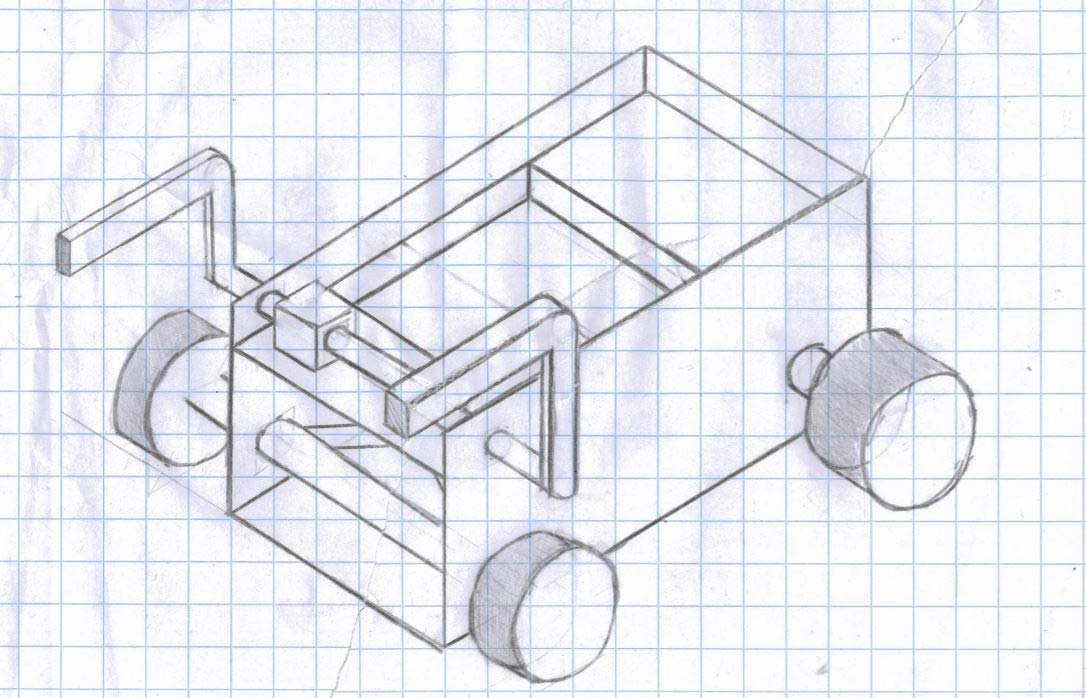
\includegraphics[width = 100mm]{04_idee_ontwikkeling/deeloplossing_mantis.JPG}
    \caption{Isometrische tekening Mantis Car}
    \label{fig:deeloplossing_mantis}
\end{figure}

De mantis car werkt door middel van grijphaken die zijn gebaseerd op de poten van een sprinkhaan, wat de naam van het concept eigenlijk al verklapt. De grijphaken worden aangedreven door een elektromotor verbonden aan de as tussen de twee grijphaken, zie \cref{fig:deeloplossing_mantis}. Deze grijphaken zouden zich kunnen vastklemmen aan het talud, en de kar zou zich op deze manier omhoog kunnen takelen.\\

Dankzij de bevindingen die zijn opgedaan tijdens het testen van het spuugmodel is er gekozen om dit concept verder uit te werken. Ten eerste bleek dat de grijphaken niet voldoende statisch gebalanceerd waren. Het omhoogbrengen van de haken vereiste een aanzienlijk moment terwijl het omlaag brengen moeiteloos ging. De motor zou dan een variabele moment moeten leveren. Om dit te voorkomen wordt een extra set haken aan de as te bevestigen, zie \cref{fig:Mantis_haak}. Dit zorgt ervoor dat de motor een minder groot moment moet leveren om de haken tot beweging te brengen en dat het moment constant blijft.
\begin{figure}[H]
    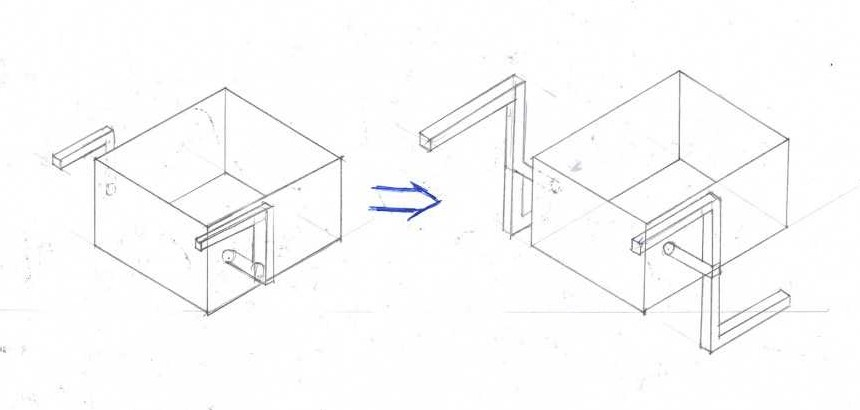
\includegraphics[width = 100mm]{04_idee_ontwikkeling/Mantiscar_armen.jpeg}
    \caption{Verbetering van de haken van de Mantis Car}
    \label{fig:Mantis_haak}
\end{figure}

\vspace{\baselineskip}
In het midden van de Mantis Car komt een schaarlift om het pakketje te ontvangen en af te leveren. De schaarlift wordt tot beweging gebracht door een stuk draadeind aan te drijven met een DC motor. Het draadeind gaat door de onderste as van de schaarlift waar een gat in is geboord van schroefdraad. Door het draadeind aan te drijven zal de schaarlift heen en weer bewegen en dus ook een verticale beweging opdoen. In \cref{fig:Schaar_boven} is dit schematisch afgebeeld.  Ook bevat het concept 2 elektromotoren: een elektromotor om de grijphaken aan te drijven en een elektromotor voor de aandrijfas. De achterste as is de aandrijfas, gekeken vanuit de isometrische tekening, zie \cref{fig:deeloplossing_mantis}. \\
\vspace{\baselineskip}

\begin{figure}[H]
    \centering
    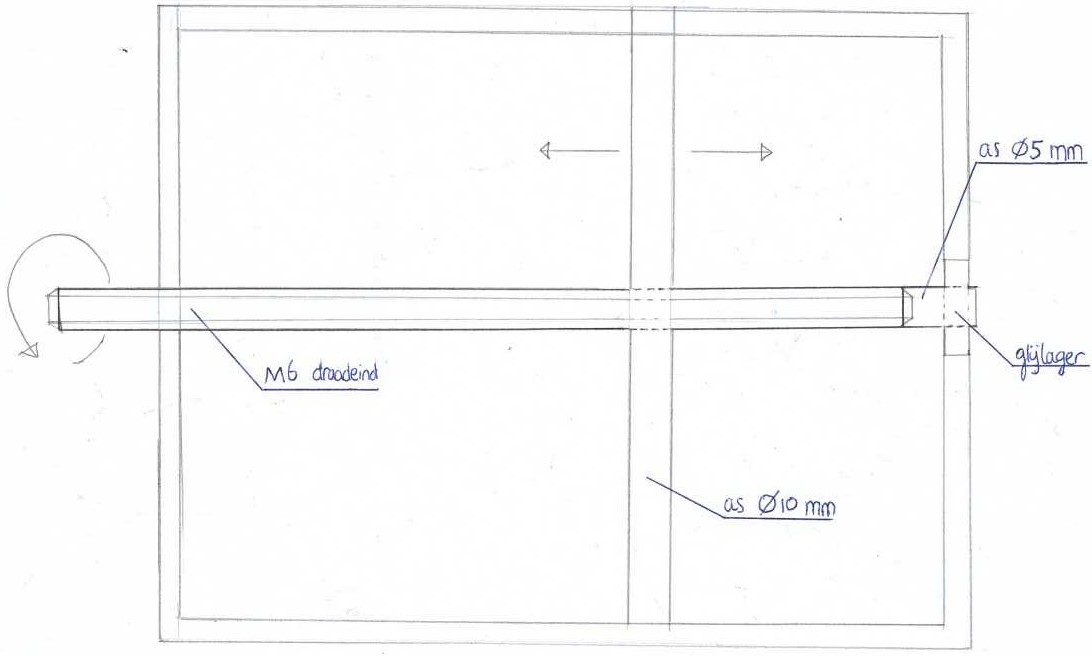
\includegraphics[width = 80mm]{04_idee_ontwikkeling/Bovenaanzicht_schaarlift.jpeg}
    \caption{Bovenaanzicht van de beweging van de schaarlift}
    \label{fig:Schaar_boven}
\end{figure}



\subsection{Concept 2: \textit{Uitschuiver}}
\label{se:concept_2_uitschuiver}

De uitschuiver werkt door een stappende beweging te maken met behulp van twee schaarliften. Als de uitschuiver in de buurt van een obstakel komt wordt de achterste schaarlift uitgeklapt. Dan wordt de voorste schaarlift over het obstakel heen geschoven door het uitschuifmechanisme. Vervolgens wordt de voorste schaarlift op de grond gezet. Door het pakket vervolgens boven de bovenste schaarlift te bewegen veranderd het massamiddelpunt van het mechanisme. Als de achterste schaarlift nu opgeklapt wordt blijft het mechanisme stabiel. Ten slotte wordt de achterste schaarlift ingetrokken door het uitschuifmechanisme en kan het pakkethondje zijn weg vervolgen. Zie \cref{fig:isom_uitschuiver} voor een isometrische tekening van dit eindconcept.
\vspace{\baselineskip}

De uitschuiver wordt aangedreven door zes stepper motoren. Onder de voorste schaarlift zitten twee stepper motoren, waardoor het ontwerp kan sturen door middel van een aandrijvingsdifferentiaal. De derde stepper motor drijft de achterste schaarlift aan, waardoor de uitschuiver ook kan rijden als de voorste schaarlift niet op de grond staat. De vierde en vijfde stepper motoren drijven de schaarliften aan door een draadeind aan te draaien. De laatste stepper motor zorgt er voor dat het uitschuifmechanisme werkt. Door weer aan een draadeind te draaien kan de uitschuiver de afstand tussen de schaarliften veranderen. Om een duidelijker beeld te krijgen van de vorm van de schaarlift kan er worden gekeken naar \cref{schaarlift_hilbert}.

Bovenop de schaarlift zit het systeem dat het pakket kan verplaatsen. Door aan het touwtje met de magneet te trekken beweegt het pakket over de L-profielen. Hierdoor kan de positie van het zwaartepunt tijdens de rit aangepast kan worden. Zie \cref{fig:detail_uitschuiver} voor een tekening van het mechanisme om dit aan te passen. 


\begin{figure}[H]
    \centering
    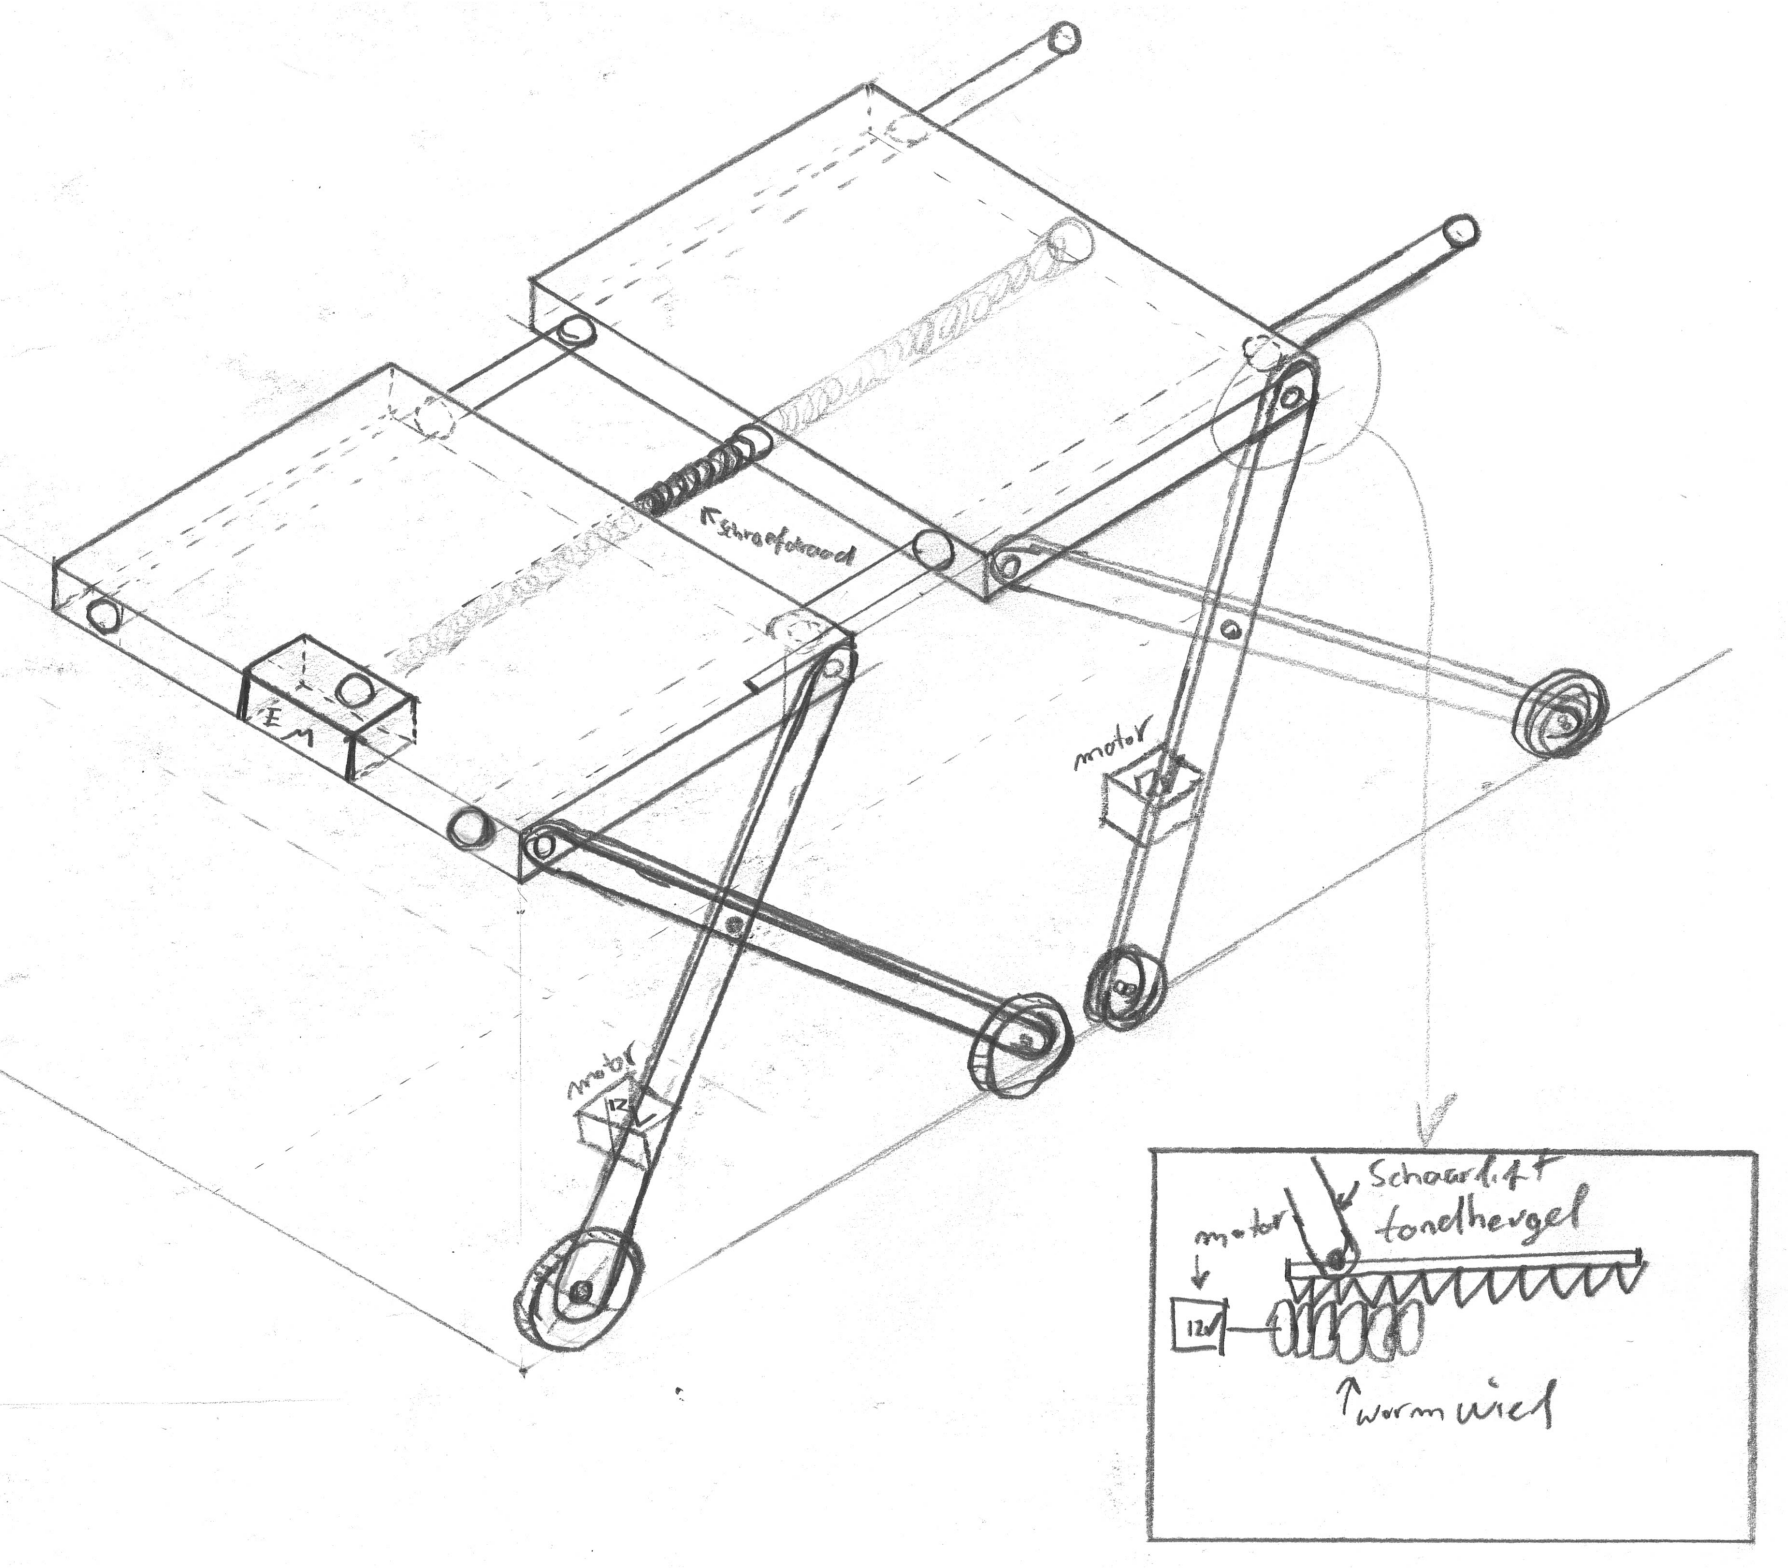
\includegraphics[width=80mm]{04_idee_ontwikkeling/isom_uitschuiver.png}
    \caption{De isometrische tekening van het concept uitschuiver}
    \label{fig:isom_uitschuiver}
\end{figure}

\begin{figure}[H]
    \centering
    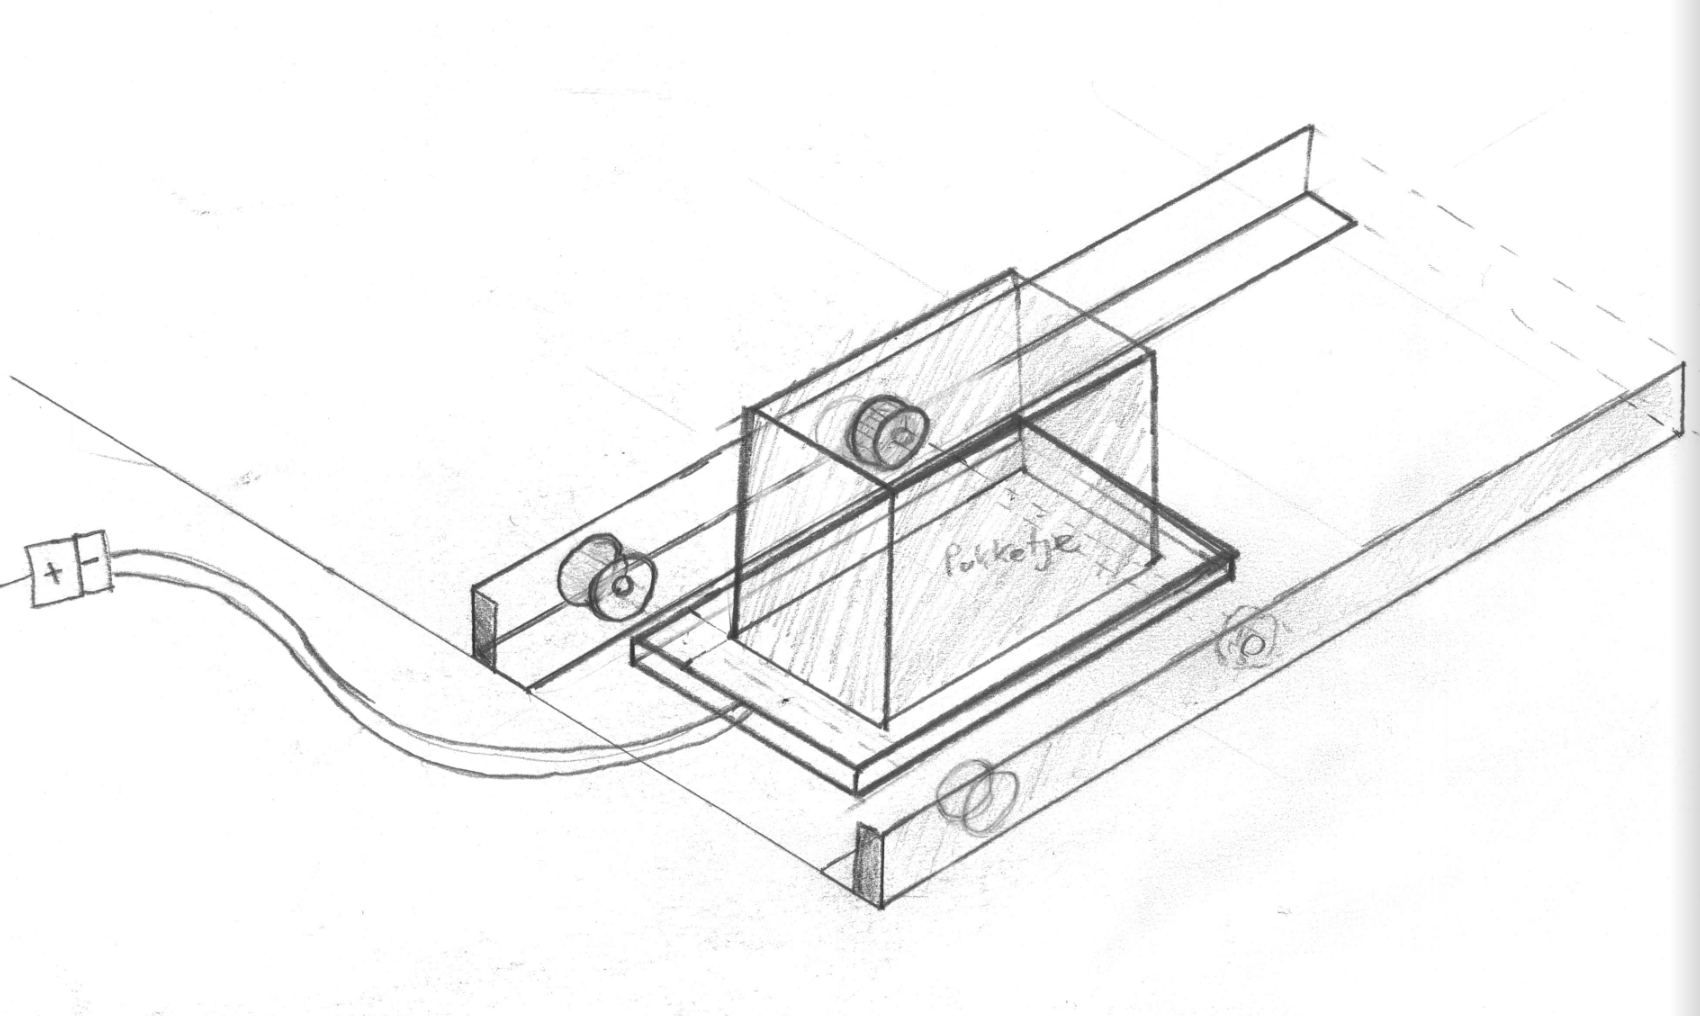
\includegraphics[width=80mm]{04_idee_ontwikkeling/detail_uitschuiver.png}
    \caption{Tekening van het mechanisme om het pakket te verplaatsen bovenop de uitschuiver.}
    \label{fig:detail_uitschuiver}
\end{figure}


\subsection{Concept 3: \textit{Inklapper}}
\label{se:inklapper}
\vspace{\baselineskip}
De Inklapper (\cref{fig:inklapper}), zoals de naam luid, bestaat uit een Plateau met 3 inklapbare wielen. Elk wiel is door middel van een schaar lift nauwkeurig op hoogte af te stellen. Het plateau heeft hierdoor de mogelijkheid in zijn geheel op/neer te bewegen, zo is het bijvoorbeeld mogelijk exact met de aanname/afgeef hoogte van het pakketje te matchen. Ook kan door de verschillende schaar liften het plateau in een hoek bewegen, ook bij een helling blijft het pakket recht. (zie \cref{fig:rechtplateau_op_helling}.)

\begin{figure}[H]
    \centering
    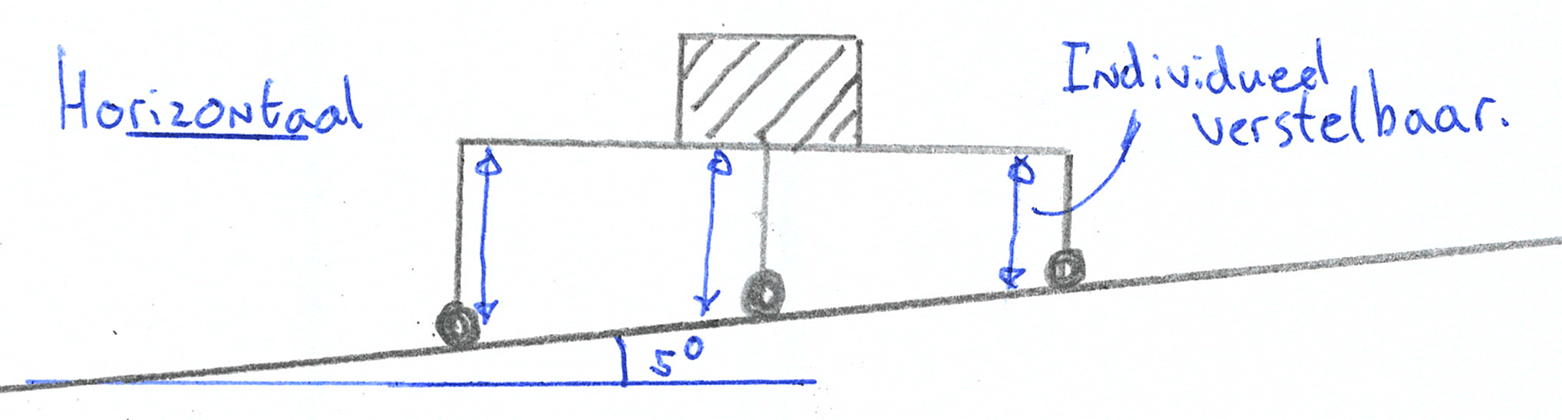
\includegraphics[width=120mm]{04_idee_ontwikkeling/Recht_onder_hoek_driepoten.png}
    \caption{Het plateau blijft recht op een schuine helling}
    \label{fig:rechtplateau_op_helling}
\end{figure}

De inklapper kan door, één van de drie wielen in te klappen zich over het obstakel bewegen. De inklapper kan zijn balans behouden door het zwaartepunt op het bewegende Plateau te verplaatsen tussen de twee overgebleven steunpunten. Het overwinnen van het obstakel gebeurd in de volgende stappen: 1 verplaatsing zwaartepunt tussen de twee steunpunten, 2 inklappen poot, 3 zich over het obstakel heen rijden, 4 uitklappen poot. Hierna herhalen deze stappen zich tot de gehele auto over het obstakel heen is. Zie \cref{fig:stappen_inklapper_met_pakket} \\


\begin{figure}[H]
    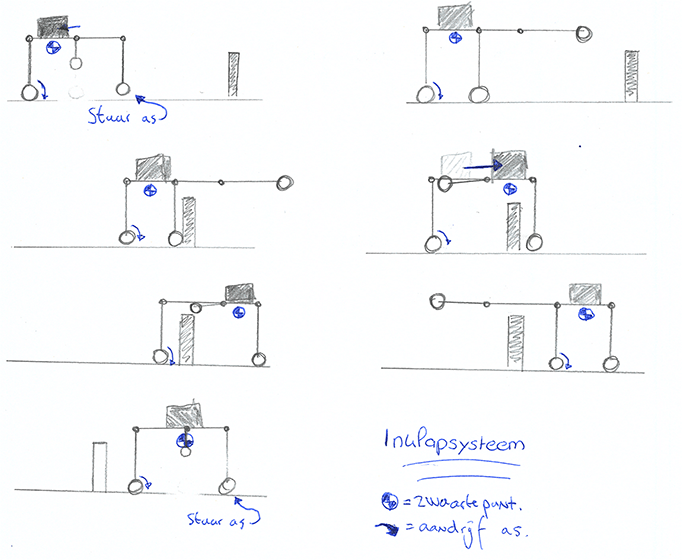
\includegraphics[width=120mm]{04_idee_ontwikkeling/Verloop_systeem_driepoten.png}
    \caption{Meerdere stappen die de in klapper onderneemt om een obstakel te overwinnen, zwaartepunt en as die het voertuig aandrijft zijn ook aangegeven}
    \label{fig:stappen_inklapper_met_pakket}
\end{figure}

De inklapper word aangedreven door de middelste en achterste as. Het is hierdoor mogelijk altijd voor te bewegen als twee van de drie poten zich op de grond bevinden. Zie figuur \cref{fig:stappen_inklapper_met_pakket} hoe er altijd een aandrijving is om over het obstakel heen te rijden. Ook word er altijd geremd op de motor, uitgaande er nooit de noodzaak is voor een grote remkracht.  Het stuurmechanisme is gebaseerd op het Ackermann-principe (\cite{Stuurmechanisme}). De voorste poot kan met behulp van een servo en een stuur mechanisme worden bestuurd. Tijdens het rijden zal de middelste poot ingeklapt zijn, hierdoor werkt het stuurmechanisme vergelijkbaar met een auto. Dit mechanisme is in \cref{fig:vierpoter_stuursysteem} uitgewerkt. \\ 

\begin{figure}[H]
    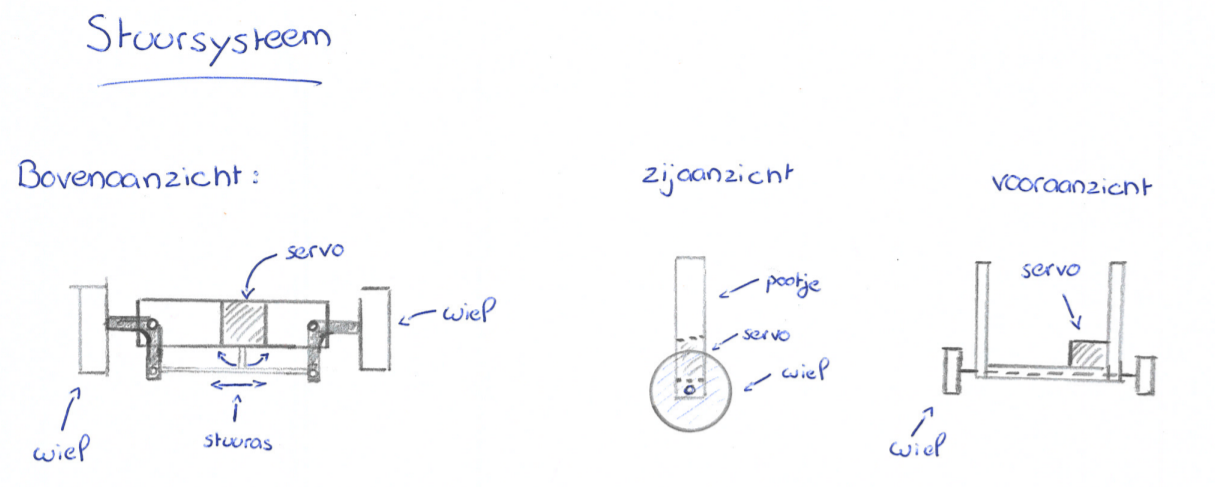
\includegraphics[width = 100mm]{04_conceptKeuze/Foto_stuursysteem.PNG}
    \caption{Concept 3, Het stuursysteem van de inklapper}
    \label{fig:vierpoter_stuursysteem}
\end{figure}

Zoals eerder vernoemd heeft het Plateau de mogelijkheid zich te verplaatsen over het dek. Aangezien het pakketje een grote massa bedraagt, heeft een verplaatsing van het plateau met pakketje direct gevolgen voor de verplaatsing van het zwaartepunt. Het plateau zit zo bevestigd op het dek dat het met weinig weerstand kan rollen, de wielen worden aan beide uit eindes geblokkeerd, zo kan het pakketje wel er af/op worden geschoven maar blijft het plateau altijd op het dek. De verplaatsing is zonder een onnodig ingewikkeld systeem maar word behulp van het touwtje met magneet verplaatst. Dit werkt nagenoeg het zelfde als \cref{se:concept_2_uitschuiver} te zien in \cref{fig:detail_uitschuiver}\\

\begin{figure}[H]
    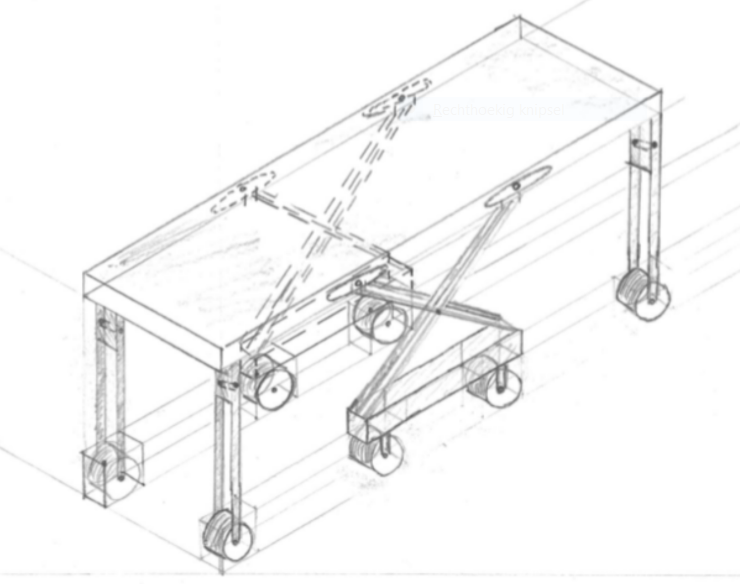
\includegraphics[width = 100mm]{04_idee_ontwikkeling/Foto_inklapper.PNG}
    \caption{De inklapper}
    \label{fig:inklapper}
\end{figure}

\subsection{Concept 4: \textit{vierpoter}}
\label{se:vierpoter}
\vspace{\baselineskip}
De vierpoter heeft inklapbare pootjes waarmee hij het talud neemt. De vierpoter rijdt naar voren door de wielen, aan de onderkant, van de vier paren pootjes.\\
De voorste twee en de achterste twee worden aangedreven door vier afzonderlijke steppermotoren. \\
De onafhankelijke aandrijving zorgt ervoor dat hij kan sturen door de wielen aan een kant, de een kant op te laten draaien dan de wielen aan de andere kant. Dit zorgt ervoor dat de vierpoter een kleine bocht met een relatief hoge snelheid kan maken.  Hoe de aandrijving werkt en waar hij is bevestigd is te zien in \cref{fig:vierpoter_aandrijving}.\\

\begin{figure}[H]
    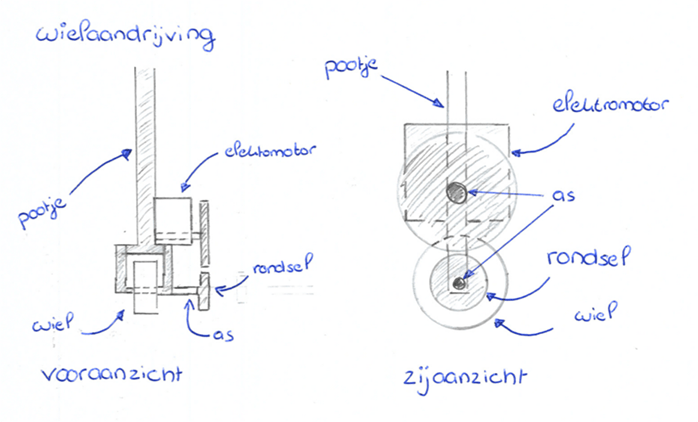
\includegraphics[width = 100mm]{04_idee_ontwikkeling/Foto_aandrijving_vierpoter.PNG}
    \caption{Concept 4, de aandrijving van de vierpoter}
    \label{fig:vierpoter_aandrijving}
\end{figure}

\vspace{\baselineskip}
Eenmaal bij het talud maakt de vierpoter gebruik van zijn inklapbare pootjes. Zijn voorste paar klappen vooruit. De vierpoter rijdt vervolgens naar voren totdat hij met zijn tweede paar tegen het talud rijdt. Nu klappen de voorste wielen weer terug en klapt het tweede paar in. Hij rijdt weer naar voren en verricht deze handeling opnieuw totdat de inklapper over het talud is. Deze handeling is te zien in \cref{fig:vierpoter_loopmechanisme}.\\

\begin{figure}[h]
    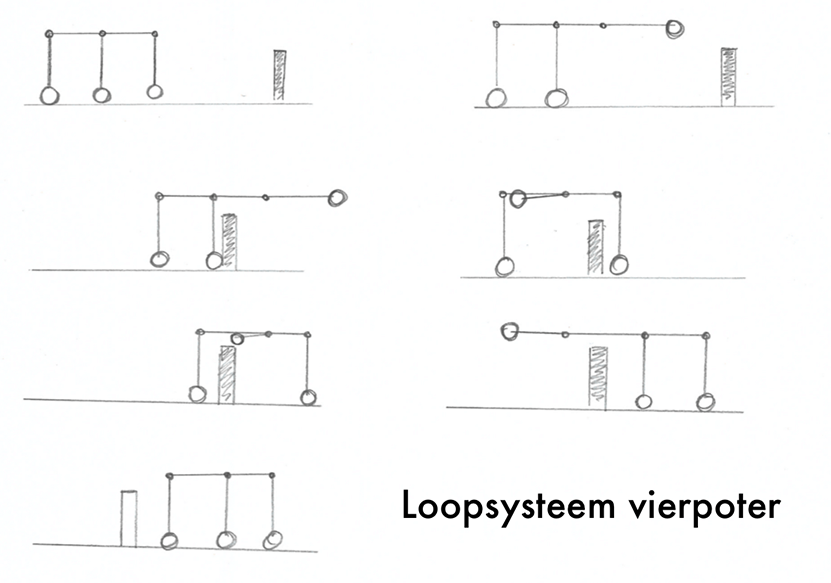
\includegraphics[width = 100mm]{04_idee_ontwikkeling/Foto_loopsysteem.PNG}
    \caption{Loop mechanisme vierpoter}
    \label{fig:vierpoter_loopmechanisme}
\end{figure}

Het inklappen van de pootjes gebeurt met behulp van een elektromotor en een tandwielen. Dit is te zien in \cref{fig:vierpoter_inklapsysteem}.\\

\begin{figure}[H]
    \centering
    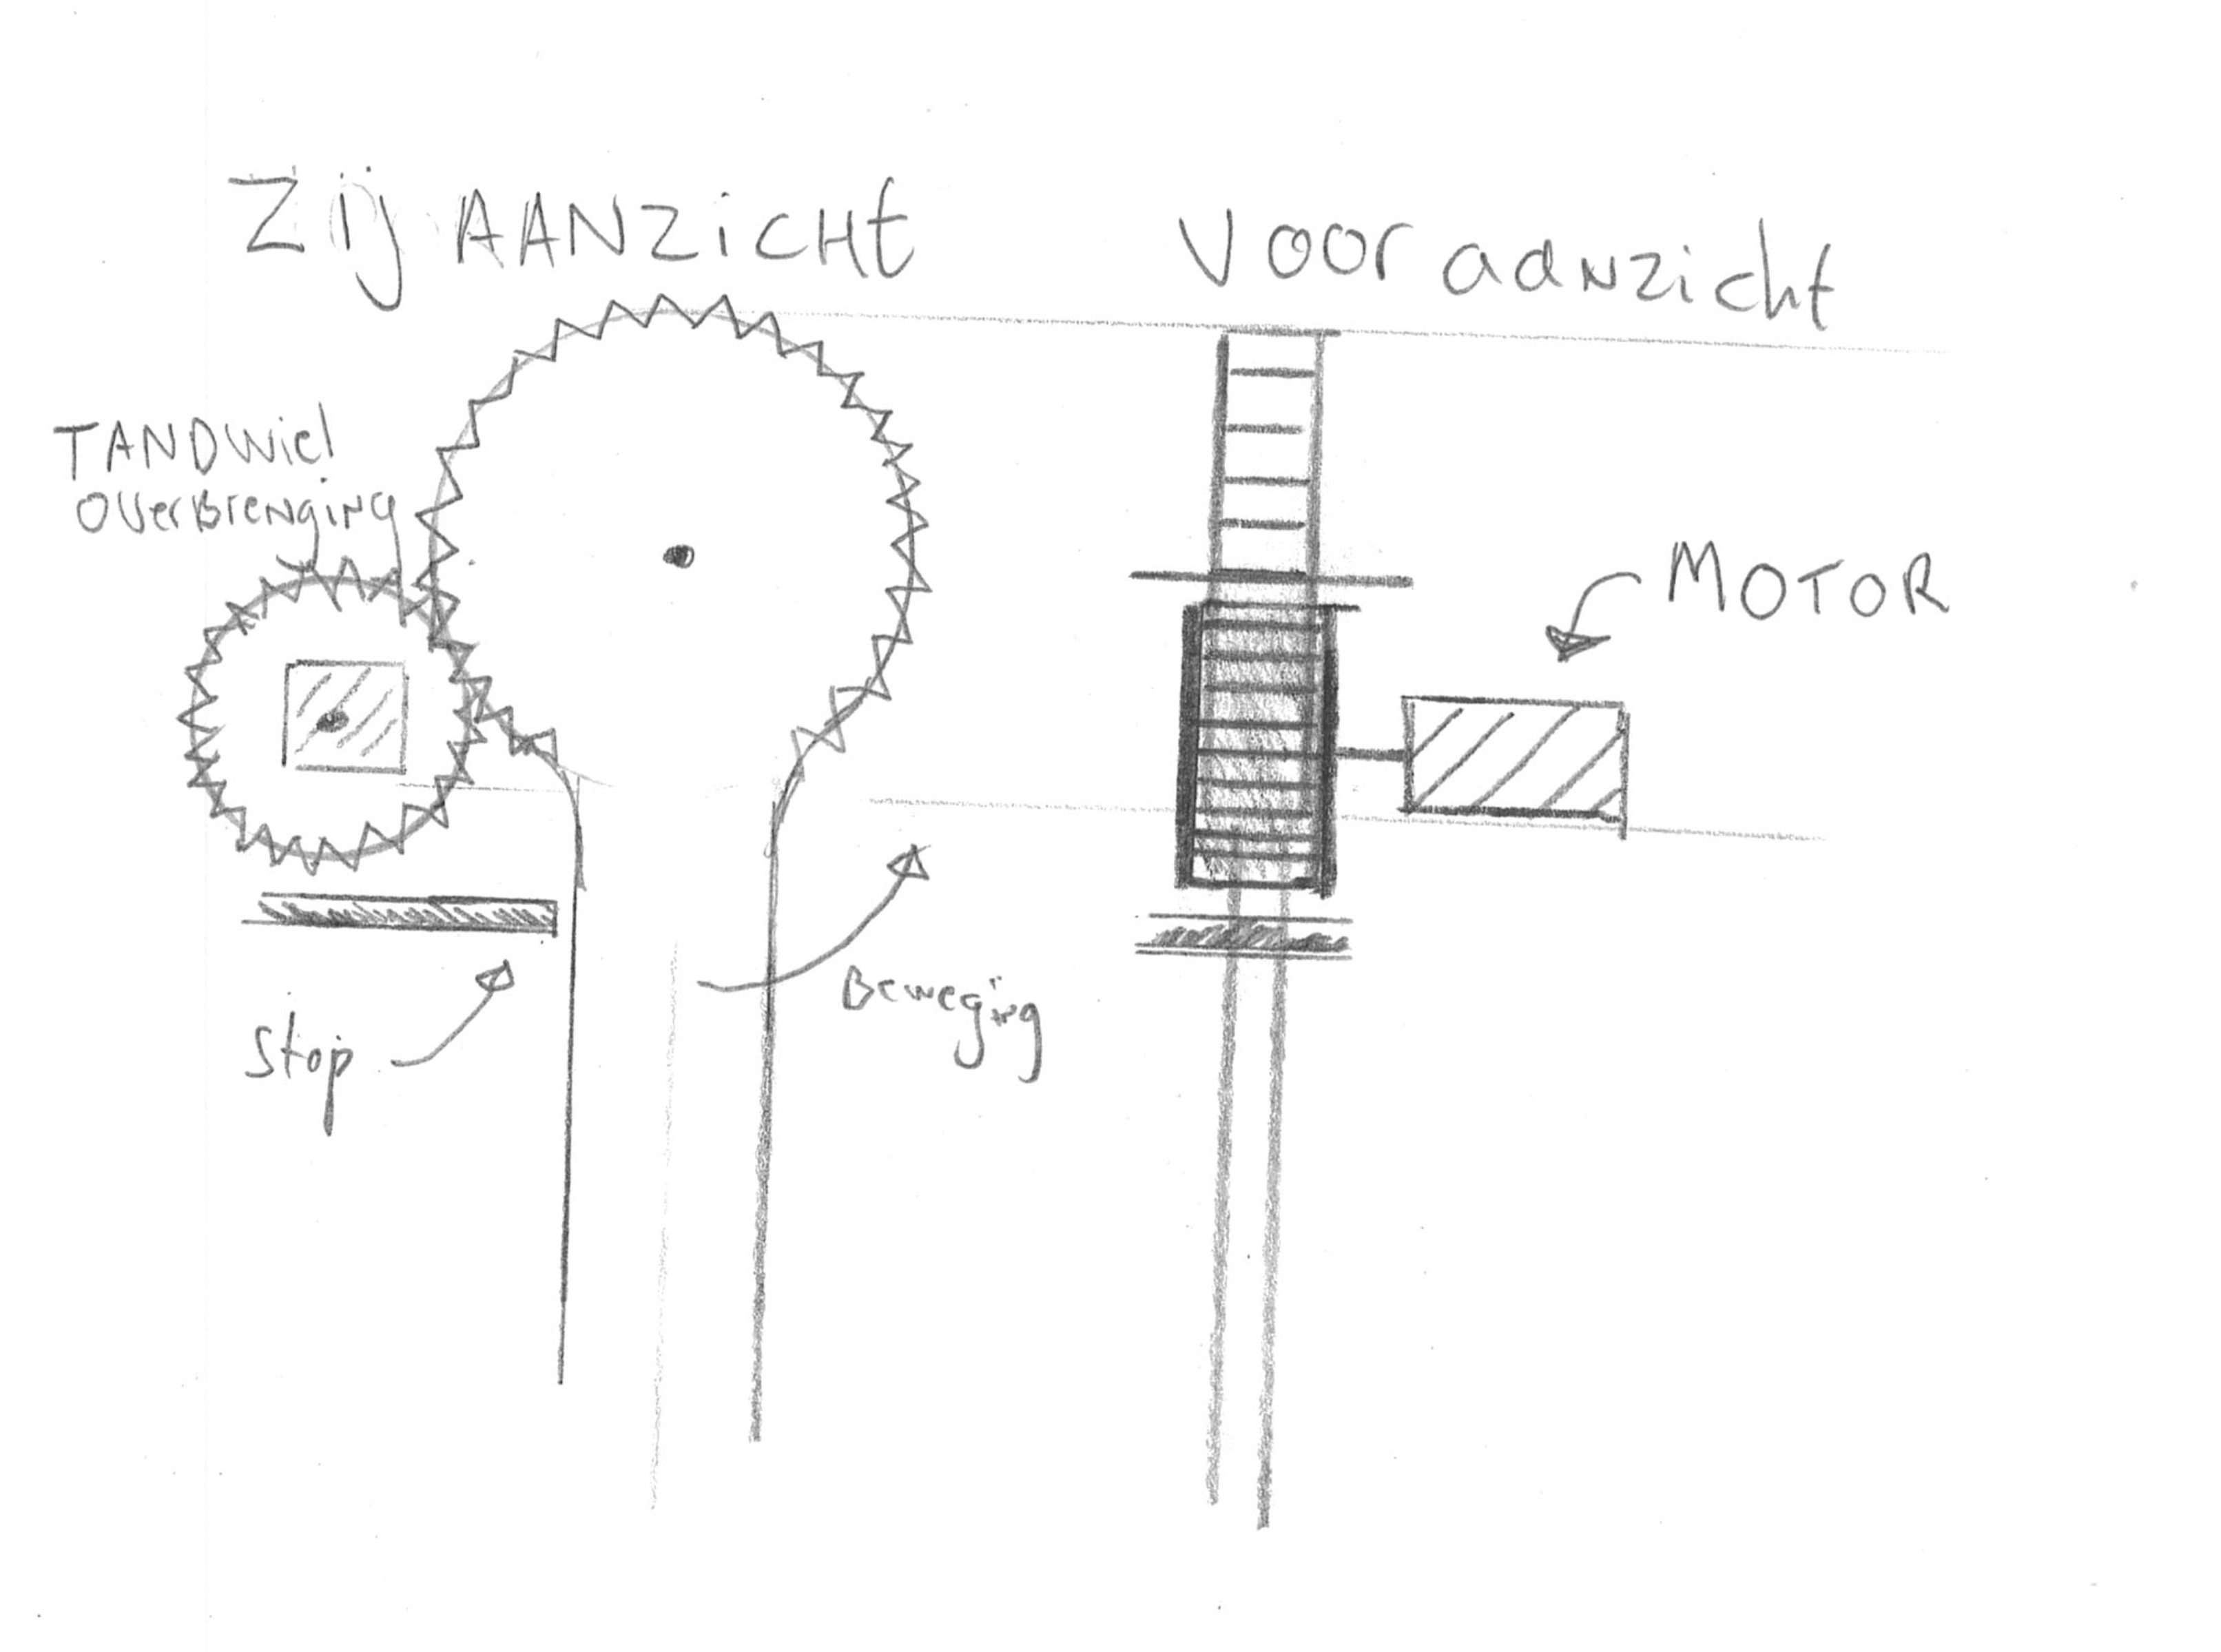
\includegraphics[width = 80mm]{04_idee_ontwikkeling/Opklapsysteem_met_tandwiel.png}
    \caption{Concept 4, inklap systeem}
    \label{fig:vierpoter_inklapsysteem}
\end{figure}

Het remmen van de vierpoter doet hij op de motor. Omdat de snelheid van de inklapper zo minimaal is en omdat er gebruik wordt gemaakt van een steppermotor is het niet nodig om remblokjes of -schijfjes toe te voegen.\\
Het ontvangen van het pakket gebeurt door middel van een rol systeem dat te zien is in \cref{fig:vierpoter_totaal}. De vierpoter is zo ontworpen dat het dezelfde hoogte heeft als het plateau waarvan hij het pakketje moet ontvangen en moet afleveren. Voor meer informatie over de vierpoter zie \cref{fig:vierpoter_totaal}. \\

 
\begin{figure}[H]
    \centering
    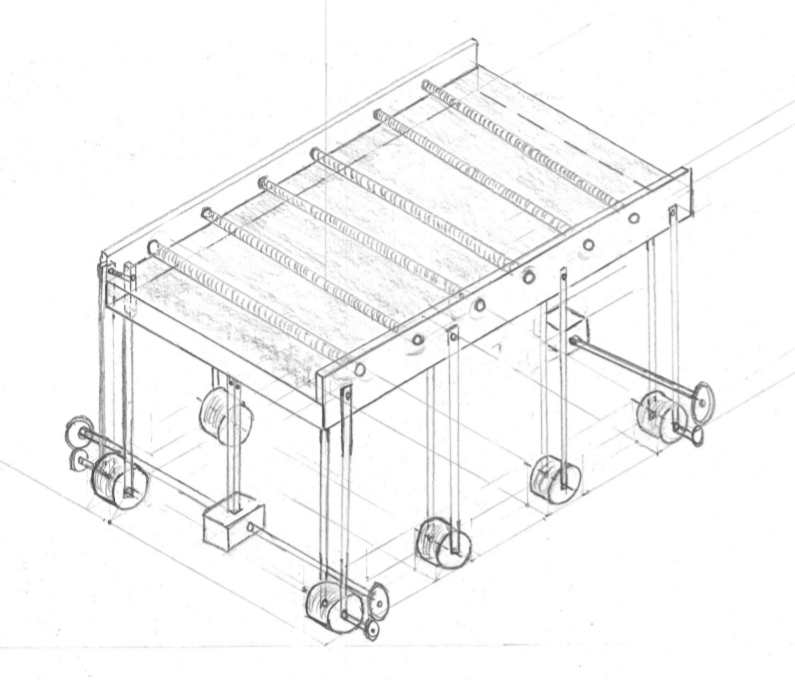
\includegraphics[width = 100mm]{04_idee_ontwikkeling/Foto_vierpoter.PNG}
    \caption{Concept 4, de vierpoter}
    \label{fig:vierpoter_totaal}
\end{figure}
